\documentclass[11pt;a4paper]{report}
\usepackage[free-standing-units]{siunitx}
\usepackage{circuitikz}
\usepackage{tikz}
\usepackage[utf8]{inputenc}
\usepackage{fontenc}
%\usepackage[French]{babel}
\usepackage{lmodern}
\usepackage{amsmath}
\usepackage{amssymb}
\usepackage{mathrsfs}
\usepackage[top=2cm, bottom=2cm, left=2cm, right=2cm]{geometry}
\usepackage{multirow}
\usepackage{url,hyperref}
\usepackage{siunitx}
\usepackage{schemabloc}
\usepackage{eurosym}
\usepackage{multicol}

\title{
\includegraphics{images/inp-enseeiht} \\ ~ \\ ~ \\ ~ \\ ~ \\ ExpoLangues \\ ~ \\ \large{The Crunch}}
\author{Benjamin Arfelis, Adrien Creusvaux,Vincent Dahi,\\ Chakib Larbi, Jean-Pascal Monvoisin,\\Vincent Petillat, Guilhem Saurel,\\Julien Tourbot, Guillaume Vota}
\date{\oldstylenums{\today}}

\renewcommand{\thechapter}{\Roman{chapter}}
\renewcommand{\thesection}{\thechapter .\Alph{section}}

\begin{document}
 \begin{titlepage}
  \maketitle
 \end{titlepage}

 \tableofcontents

 \chapter{Team}
  \begin{description}
   \item[Project Leader :]Tourbot Julien
   \item[PMO :]Petillat Vincent
   \item[Secretary :]Saurel Guilhem
   \item Arfelis Benjamin
   \item Creusvaux Adrien
   \item Dami Vincent
   \item Larbi Chakib
   \item Monvoisin Jean-Pascal
   \item Vota Guillaume
  \end{description}

 \chapter{Organisation}
  \section{Proposal}
Hello,

~

We finaly made the ExpoLangues group.

We will deal with the historic and cultural clash between France and England.

~

The members of the group are :

Tourbot Julien (Project leader)

Petillat Vincent (PMO)

Saurel Guilhem (Secretary)

Larbi Chakib

Vota Guillaume

Arfelis Benjamin

Dami Vincent

Monvoisin Jean-Pascal

Creusvaux Adrien.

~

Thanks for noticing it.
  \section{Minutes}
   \subsection{First meeting}
In this first meeting, we talk with the client about the choice we made about our subject. She thinks it was an original an interesting idea because of the possibilities we had with the choice of activities.
We talked about the activities we planned to do, and it seemed that all were fine.

   \subsection{Second meeting}
We talked with the client about the progress we made since the last time we met. The client didn't make us special remark about our work, she seemed to think it was fine.

  \section{Gantt Chart}
    \begin{center}
     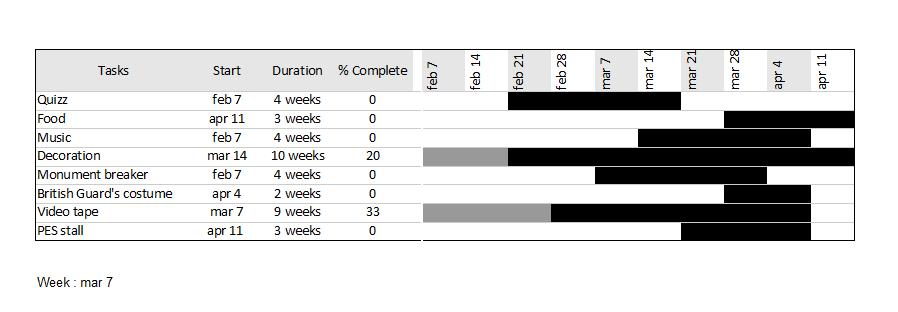
\includegraphics[width=15cm]{images/gc1}
     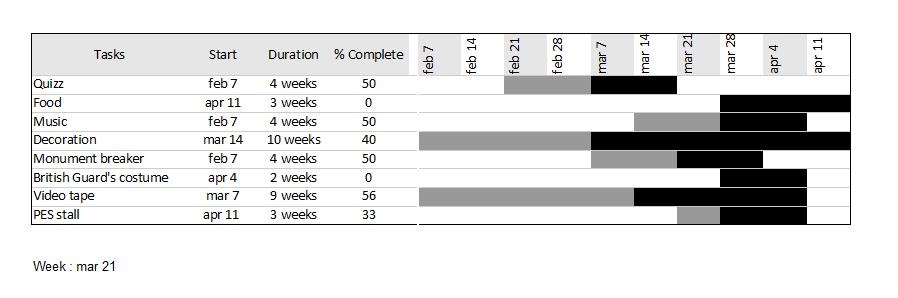
\includegraphics[width=15cm]{images/gc2}
     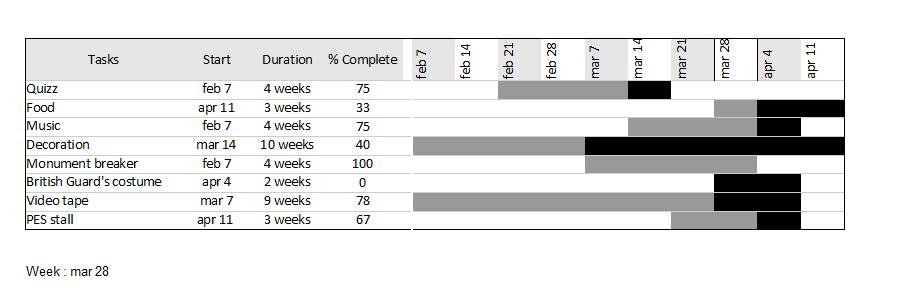
\includegraphics[width=15cm]{images/gc3}
    \end{center}


 \chapter{Personnals inputs}


  \section{Benjamin Arfelis}
\newpage
  \section{Adrien Creusvaux}

I chose this subject because I found the idea to make a comparison between France and England really relevant. I think this topic is open since the points of comparison are numerous. I mean that there is a lot to talk about such as sport, customs, music, weather, food and so on.
Moreover, when we thought about this theme, it has seemed to be easier to find animations, activities so as to attract and entertain the visitors.

~

Project Team Organization:
The project leader had to organize some meetings to estimate the project’s progress. At the end of these meetings we made a brief summary to evaluate the amount of work remaining.
Finally, the report editor had to gather the different parts of the final report.

~

Our ExpoLangues was based on two steps.
The first one consisted in thinking about all activities that we will be able to do.
Then, each of us chose an activity.
I had to make a short and funny quiz to attract visitors and to create a good atmosphere. Here is the quiz:

% TODO Quiz...

 had to cope with some problems especially to find decoration and to create an atmosphere in the room.

~

i learned to manage a given amount of time so as to respect a deadline and to be ready for the day d.

~

We used electronic equipment such as computers, video cameras and projectors that we have borrowed to the Service Langues.

We also used basic kitchen material to cook traditional meals from France and England.

~

To attract visitors, we displayed flyers everywhere and we made a marked route because our room was quite hidden (B007). Moreover, we sent a message on a famous social network.

~

The activities were chosen to have a good interaction with the visitors. We had a monuments breaker where you chose to destroy the Big Ben or the Eiffel Tower made with cans. We had darts with two targets: Queen Elizabeth and President Sarkozy. We had a quiz with funny comparisons between France and England. We had a Playstation so as to play football match France versus England. We had French and English music. We had an English guard and we could take photos with him. 

~

I think that we have filled our objectives except for the atmosphere which was not as good as our expectations. Indeed, I think we didn’t have enough decoration.

I wish we had had a little budget for this project in order to buy a minimum of decoration (because we didn’t want to put too much money for decoration). 


\newpage
  \section{Vincent Dahi}

    All of this long and hard work about “expolangue” has begun when we were in class with Bob. Indeed, we discovered that we have the difficult mission to choose a subject with no restrictions. The main difficult was to find a subject which shall allow the implementation of recreational and funny activities. 

Moreover, Bob has had the habit to talk us about rugby and the fact that since the creation of this sport, there is an important rivalry between our countries.
That is why, we decided to talk about the differences between England and France with different point of view, such as: sport, culture. We chose it because we thought that many people could be interested by this topic, and feel concerned. The possibility to realise lot of practical activities confort us into our choice.             

~

For the logistic point of view, I think we had a good team, motivated by the choosen subject, and well organized, because rapidly different activities came easily to our mind, allowing us to take decisions and to target tasks to achivied.
However, several difficulties bother us, especially for the realisation of our activities, slowing down our progration. For example we had a problem to create a “coconut shy” with famous monuments. But with a little of ingenuity we overcame that problem.
Thus, I can say we only had practical problem 

~

So as to create an atmosphere favourable for the big confrontation, we had to find decoration, costumes and food characterizing both countries. Moreover, we wanted to project a film so we had to make a video editing, and we needed to find a projector and speaker.

~

I think maybe the most important difficulty of the exhibition was to attract visitors. That is why, we decided to put several notices into the different building of the school, especially into the B building. We decided to stand an typical English guard near the entry to create curiosity and giving the desire to come see our exhibition.        

~

For us, activities had a huge importance in our exhibition because we thought that it was what will allow us to attract the visitors to interest and to make them stay as long as possible with us. That is why we developed several activities, such as:

 A “coconut shy” where you could choose to destroy a French or English famous monument, the Eiffel Tower or Big Ben according to your preference. Of course after the destruction you had their descriptions. 

A quizz so as to learn you the cultural difference between France and England while having fun.

Darts which was the activity I had to present. There were two portrait that I had drawn which represent Nicolas Sarkozy and the Queen Elisabeth. I chose them because they represent their countries. The goal of this game was that you had to aim parts of their body with darts so that I can tell you anecdotes on these two characters. For example, if you aimed at Nicolas Sarkozy's head, I spoke to you about his school level. 

A video game of soccer so as to confront the French team against English team, to  strengthen the atmosphere of confrontation.

I think our activities performed well their role, because many people were interested in our presentation and took pleasure to participate to our activities.  

I think the various objectives that we had settled for our project, as to attract most possible visitors, make them discover the French or English culture by funny activities, while avoiding them boredom, were performed, because several person appreciated our activities. But we had to admit that it was difficult to keep the attention of our visitors when we tried to tell them our explanations.. So we could say that we had a lot of good commentaries about our exhibition, especially for the activities.

Moreover, we did not want to pay a lot of money for our project that is why most of our activities could come true without needing to buy materials. Only our creative spirit was put in contribution. On the other hand, we wished to make discover culinary specialities of both countries, we were thus obliged to buy ingredients. But we knew how to limit the cost. Fortunately, the professors knew how to help us for the decoration and disguise, by lending us objects and costumes.

For a time point of view, I could say how we are all in the same state of mind, that was easy to create our exhibition rapidly.   

~

  I think the only critique for the progress of “expolangues” would be that there were too many projects which taking place in the same period and during a too short while of time, what made that the visitors did not really have time to follow a project which they estimated, if they wished to discover also the other projects
However I think that.was a very good experience of a team work, and a very good way to discover how to manage a project. 

\newpage
  \section{Chakib Larbi}

    The first time that Bob Hendry talked to us about expolangues, it was during Six Nations ( rugby tournament), only one week before the “Big Crunch”. The Crunch is the big game between France and England. These teams are the best in northern hemisphere so this game is very attractive. We are in Toulouse so people love rugby    . This is why we choose this subject. First we wasn't very concerned by the  subject : no idea, classroom B007... The beginning was hard. 

~

    Then we had our first client meeting. We presented our subject to the professor and she was very excited. But she said that we didn't do anything. So she said that we will have to be more efficient during the second client meeting.  We needed ideas and a lot of animations in order to amuse people. Each person of the group proposed one idea for the expolangue. I like cooking and we saw in others expolangues that there always was food. So I wanted to compare French and English food. 

~

    Others had to do little games about history, sport and policy. We didn’t focus on sport only. We had dart game with Nicolas Sarkozy and Queen Elisabeth. In the same time we gave anecdotes on them. Moreover we had Can knockdown : people had to destroy Big Ben and the Eiffel Tower. This game and the quiz talked about the history of these countries.  For sport one made a video resuming big football or rugby games. For me I searched recipes easy to make. So I chose delicatessen and cheese for French food and pancakes and milkshake for English food. I didn't forget the real English tea. It's easy to make and not very expansive. 

~

    After the two others clients meeting we were ready.  The Big Day came, the sun was shining and we finished to prepare our classroom at 13:30 P.M. It was very funny for people to destroy Big Ben and the Eiffel tower ans to “hurt”  the Queen and Sarkozy.  People were captivated by the video because it was good memories with football and rugby world cup.  Unfortunately people are especially interested by food. So they were disappointed when we didn't have food anymore. People really liked pancakes and milkshakes because they were hot. At the opposite the tea wasn't very appreciate. I added a last animation because I found a rugby ball the morning and I built rugby post. Thanks to that people could shoot rugby penalties. 

~

    I think or I hope that professors were very happy to see these animations. A good point was to be able to explain what we made in Spanish ( 2nd language) even if it's quite hard. I was disappointed because people focus on food and drink and they are not very interested by what we can learn to them. Moreover this expolangue cost about 20\euro{}. But no money was given for this project. I think that we could give about 30\euro{} to each group but only for animations, not food. About the classroom we were unfortunately in room B007 because we sent our subject too late. These room B00. Are not very attractive for people and professors. And when you know that your mark depends on influx, it's not very fair.

~

    For next year I will try to promote groups without food. I learned new vocabulary. I improved my oral comprehension and expression. Work in group is very interesting. To finish I think that the most interesting is the several weeks that you have to prepare your expolangue because the Big Day is not very useful when people only want food. 

\newpage
  \section{Jean-Pascal Monvoisin}

We had the idea to choose this subject, because as everybody knows, there is a very big rivalry between France and England for a long time in of numerous domains, and we decided to exploit this rivalry to create activities and to see who is the "best" and who would have most success beside to the students.

~

To attract the visitors we put posters almost everywhere in the school, but principally in the places the most frequented as the Hall C and the foyer and in the hall of the building B because the expolangue unwound here. Then to interest people and to make them stay, we had food and drink, music and varied activities like darts, “chamboule tout”, the games console or also a quiz.

~

As we indicated previously, the main activity were dart or it was necessary to choose at which head of state we wished to aim (we had the choice between the queen of England, the queen Elizabeth II, and the president of the French republic, Mr Nicolas Sarkozy), then we had the "Monument Breaker" where we had to choose which monument to destroy, on principle of "chamboule tout", between the Eiffel Tower and the Big Ben. We also had a computer where we could make match France versus England on the game Pro Evolution Soccer, a game very appreciate in the field of the football. Then we had a place where was proposed various English food and French food : for the English food we had for example Milk shake, gele and for the French food we had of the sausage and the pâté (we played mainly on the cliché that we can have of both nations). Finally we had a short movie which turned in buckle and which told the exploits past of both national teams in the field of the football and of the rugby. We had also a quiz about the both nations and an authentic English Guard which did not move whatever we made in front of him (even if he sometimes smiled) and with whom we could take pictures.

~

The visitors appreciated the activities in a general way. What had the most success is the food, but the other activities also interested people. When a person tried an activity, he tried generally every others activities then.

~

The main problem concerning our expolangue is that not many people came because of the situation of the room. Indeed, we were in B007 and although we put a lot of posters and road sign people did not come to our room. The stream visitors was by wave, so sometime there was too many people in one time, or sometime practically nobody.

~

Our project did not us cost many money, indeed we knew how to manage with our means. The only spends that we had was for the food, it cost to us about 3\euro{} by person. Then we were able to build the rest of our activity without spending money, by using old materials or thanks to what English professors gave to us, like a red jacket for the English Guard, cans for the “Chamboule tout” or some decorations for the room. 

~

The main default of the expolangue is that we do not have a lot of time before the presentation to organize all the room. I think it would be preferable to have no class before the presentation to have the time to prepare the room correctly.

Moreover, we can notice a problem for the expolangue which is that it is entirely prepare in French, so we do not speak a lot English during this English class.

Otherwise the project in itself learn us to organize ourselves to build a project.

\newpage
  \section{Vincent Petillat}
\newpage
  \section{Guilhem Saurel}
  
    On this "Expolangue", we democratically decided to make something about the strong tradition of competition between France and England in many subjects.
We could also have choose Star Wars as theme, so that the atmosphere would have easily been funnier... But we found more different attractions and we thought that the teachers will be most interested bye "The Crunch". In my opinion, I probably did a better preparation work on Star Wars because I'm more interested by it, and I had interesting ideas about what to do.

~

So our subject was to compare France and England on several themes, and I chose to be responsible of the music, because I saw here a way to improve my culture of the music in these countries during the last half century.

The idea was to play a famous song of each countries from each year since the 60's. The first playlist I made was made with the different charts of both countries, to compare the atmosphere of what has been listen through the years, but it appeared that there were more foreign songs which was loved in theses countries than local songs.

So I had to make another one playlist, with only local songs, but I didn't succeed in making something which really represents all the different periods since the 60's : 
\begin{itemize}
    \item For the English side, I found too many songs of the Beatles ans two songs of Queen rather than many different artists
        \item About the French songs, I don't really know a lot of successful songs older than me...
        \end{itemize}

        Here is the playlist :
        \begin{multicols}{2}
         \begin{description}
          \item[Indochine :]J'ai Demandé à La Lune
          \item[MC Solaar :]Hasta La Vista
          \item[Jean-Jacques Goldman :]Je te donne
          \item[Daft Punk :]One More Time
          \item[Emile \& Image :]Les démons de minuit
          \item[Pow Wow :]Le Chat
          \item[Manau :]La Tribu De Dana
          \item[Queen :]Bohemian Rhapsody
          \item[Queen :]We Will Rock You \& We are the Champions
          \item[The Corrs :]Breathless
          \item[Fatboy Slim :]Praise You
          \item[The Animals :]House Of The Rising Sun
          \item[The Beatles :]She Loves You
          \item[The Beatles :]I Wanna Hold Your Hand
          \item[The Beatles :]Hey Jude
          \item[The Beatles :]Let it Be
         \end{description}
        \end{multicols}

        ~

        In fact, the main problem wasn't exactly about the playlist itself, it was that I didn't made a lot of communication about why there was this music, and the improvement of the ambiance I expected never occurred. People where just earing that there were a music, but they hardly understood it.

        But I think that this was a general fail about our Expolangues : I saw people who didn't really realise that we always were making comparisons, even with games or food.

        ~

        In spite of these few problems - the ambiance and the people who didn't understood what we were exactly doing -, I think that our Expolangue was a success, because most of the people who found our little room had a lot of fun with the dart game and the monument breaker, and learnt many things from the quizzes (that I particularly like), the videos and the sheets about Sarkozy and Elizabeth II we put on the wall (which are in annex). It was also really great to compare both food, because Chakib Larby cooks really well (his milk-shake was perfect).

        And for the food comparison, I brought some English Tea I bought in England and I really didn't like. I'd never understood why English people are so well known about their tea if it was so disgusting, so I decided to share the question with the different people who came. And a lot of them were very surprised that this awful tea was the famous English tea, but I was also very surprised that some of them, both English and French, really like it.

        ~

        The strangest thing of this Expolangue was that I was certain that both French and English rugby supporters would have cry their love of their team, seeing the video, the shirts, the flags and the little game we prepared with a small balloon, but it didn't happened.

\newpage
  \section{Julien Tourbot}
    At the beginning we were interested by two subjects. We had to choose between Star Wars and the Crunch : the rivalry between England and France. We voted and chose the Crunch. The group thought that this subject would more interest people than Star Wars, and also that we could do more interactive activities about the rivalry.

~

    Then we decided that it would be a good idea if I was the project leader because of my last year experience in expolangues. The harder part of my job was most probably to motivate my team mates in order to respect the deadlines we set.
First, we had to find activities for our expolangues. I will develop it in a following paragraph.
We didn't have problem to share the different activities between the team members. We decided that the ones who weren't responsible for anything will deal with the decoration of the room we chose. Then everyone who were responsible for an activity had to make research about their subject, and when they finished it we set the deadlines and the orders we will make the different activities.
To be honest, the organization of our expolangues went well. We just sometimes have some motivation issues.

~

    First, we chose to make five interactive activities in addition to a video which was projected on a wall,  the music and the food. And to be sure they were people at our expo, we put posters telling what and were was our expo in the school.
The video was a compilation of the different sports meetings between France and England, and particularly in football and rugby. It was done to add dynamism to the atmosphere. We also cooked English and French food.
The music was part of famous English en French bands.

~

    \subsection{The monument breaker (coconut shy)}
We made two famous monument with cardboard paste on cans : the Eiffel tower and Big Ben. The  purpose was to shoot them down with a ball. If people wanted, the responsible of that activity could give them details about their history, and there were posters which dealt with that. 
We thought that could be a funny way for people to discover a little bit more those two famous structures ; and by letting them choose which one they want to destroy, to highlight the rivalry side.

    \subsection{The darts game}
At the very end, we decided to add an other activity to our expolangues : a darts game. We drew the French president N.Sarkozy and the English Queen on two big pieces of cardboard. The aim was to shoot them with the darts. There was also explicative posters dealing with the Vth French republic and the history of the English royal family. As for the monument breaker, we would like to make people learn a part of the politic life of those two countries, and to highlight the rivalry side again.
The public we had had well reacted to those two first games because they were easy to understand and funny. But on the other side, they didn't care enough about the history of the monuments and the politic. 
So I suppose that the activities were not well thought.

    \subsection{The quiz}
In order to reinforce the instructive side, we had the idea to make a quiz which dealt with general things or events in France and England.
Just a few visitors tried this activity because they thought it was not funny enough.

    \subsection{The Pro Evolution Soccer stall (football video game)}
We put a PlayStation stall in a side of our room. The aim was only to give fun to the visitors who wanted, by playing short football matches. This stall was always full, so I guess that people enjoyed it.

    \subsection{The English guard}
In order to add some fun to our expo, we had the idea to play the role of an English guard. We made the costume by our own hands, and seeing the reaction of the visitors I think it was really a great idea. There were many of them who wanted to make a photo with him.

    \subsection{Conclusion}
    To conclude about the success of our expo, I think it was fine but not as well as we hoped. Maybe the room we were (B007) was a factor, but in my own opinion it's because we didn't really made a good atmosphere.

~

    I'd like to conclude with my personal opinion about the expolangues. In general, I think it was a little to long. I had issues to stay motivated throughout the project. Moreover as a project leader it was sometimes boring to repeat again and again what to do to my team mates. On the other side, I think it's a good experience to improve my managerial skills, and I had fun too.

\newpage
  \section{Guillaume Vota : "The Monument Breaker"}
   \subsection{Realization}
    When we chose the theme of our Expolangue this stand was one of our first ideas. The goal was to make a real clash between the two sides. It was linked to one other idea which was to make a stand with different typical small game, but this idea was replaced by the dart game stand. After few researches we found that the equivalent of the French “Chamboule Tout” was the “Coconut Shy”.

~

    A coconut shy (or coconut shie) is a traditional game frequently found as a side stall at funfairs and fêtes. A player buys three wooden balls, throws them at a row of coconuts balanced on posts and wins each coconut successfully dislodged. In some cases other prizes maybe won instead of the coconuts. But coconuts were too expensive and less easy to find so we decided to make it in a different way. So we decided to use the French version.

~

    In France, the game is called “Chamboule-Tout”.A Player throw 3 balls balls at empty tins. It’s very popular on school-parties called “Kermesse” were most of time the balls are curled socks. In German-speaking countries is called “Dosenwerfen” and is some time played in a professional way on fairs. So we started thinking how to create the perfect “Chamboule-Tout”. In the first time we decided to build “The Eiffel Tower” and “Buckingham Palace”. I was chosen to do everything linked to this activities when we make the team and chose roles.

~

    Building the monuments wasn’t the hardest part of the job! It was to find how make monuments with tins and found theses tins. Thanks to our Client who gave us the tins I used, I had time to realise the monuments. When I was building the Eiffel Tower I realise that it was easier to build something high. So I took the “Big-Ben” instead of the “Bucking Palace”. I also had to say few things about the monuments when people won the game so I made researches and create small cards (and posters too):

\begin{description}
 \item[Name :]The Eiffel Tower
 \item[Date :] 1889
 \item[Construction Time :]2 Years
 \item[Main contractor :]Gustave Eiffel
 \item[Notes :]
%TODO moche

\begin{itemize}
  \item Tallest in the world from 1889 to 1930
  \item 3 Levels, Restaurants, Elevators
  \item More than 200 000 000 people have visited the tower since its construction in 1889, including 6 719 200 in 2006. The tower is the most-visited paid monument in the world
  \item Hitler conquered France, but did not conquer the Eiffel Tower
  \end{itemize}
 \item[Reproduce/inspiration :]


 \begin{itemize}
  \item Blackpool Tower (Blackpool-England)
  \item Tokyo Tower (Tokyo-Japan)
  \item Eiffel Tower (Las Vegas, Nevada-USA)
  \end{itemize}
\end{description}
% TODO : BOXES
\begin{description}
 \item[Name :]Big Ben
 \item[Date :]1859
 \item[Construction Time :]1843-1859 (Part of a huge project)
 \item[Main contractor :]Charles Barry
 \item[Notes :]


  \begin{itemize}
  \item Largest four-faced chiming clock
  \item Third-tallest free-standing clock tower in the world.
  \item Big Ben is actually the nickname of the largest bell in the tower: the Great Bell
  \item Symbol of the United Kingdom and London, particularly in the visual media
  \item The clock and dials were designed by Augustus Pugin.
  \item The clock chimes midnight to celebrate the new years. It’s a famous event in England.
  \end{itemize}
\end{description} 


\subsection{During The Expolangue}

\begin{center}
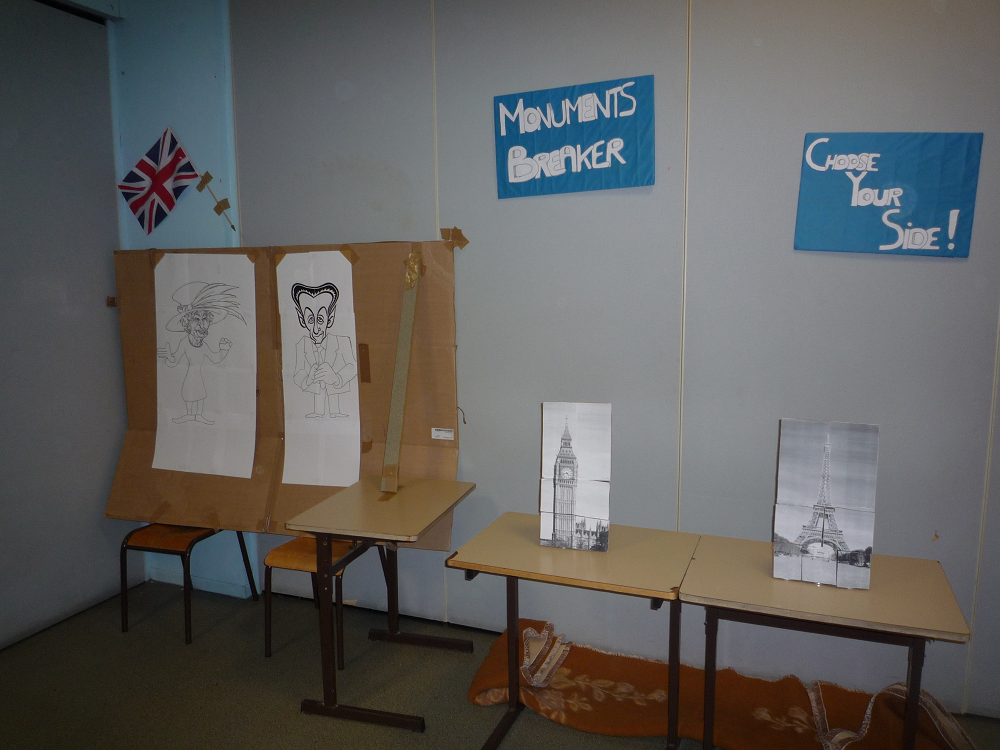
\includegraphics[width=15cm]{images/MB}
\end{center}

    This stand was just next to the dart game, so visitors will have a double chance to choose their side between France and England; personally I had already chosen my side by dressing as the typical Frenchman. But instead of the dart game, my stand doesn’t seem to be obvious to the visitors. So I spent most of my time attracting people to the Stand or explaining them what to do. I realise that people doesn’t read the poster I have made and pasted on the wall or that there were not clear enough.

\begin{center}
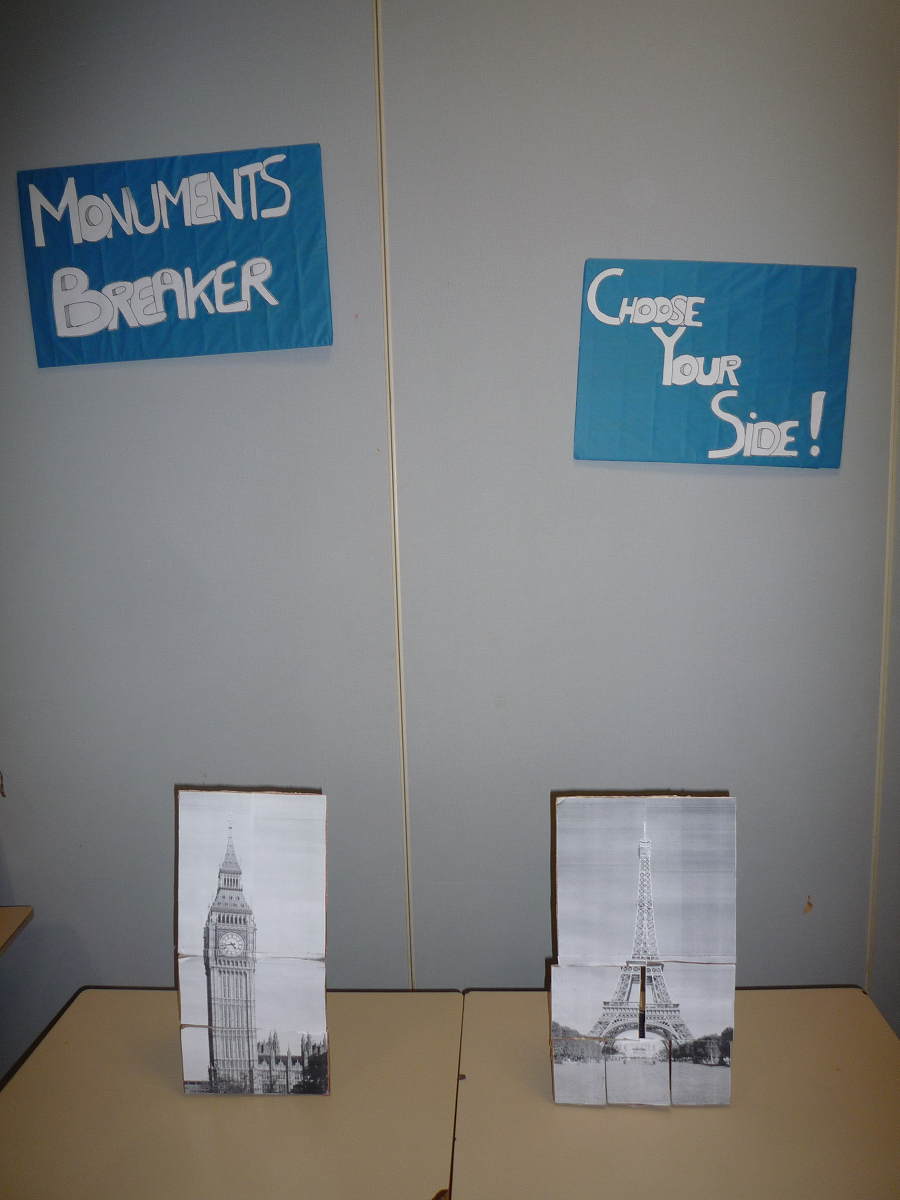
\includegraphics[height=15cm]{images/MB2}
\end{center}

    Despite the fact that a lot of people don’t try my stand because I was already busy explaining to other people, it had some success. In the beginning I tried to count the number of destruction for each monument but I lost the count after about 1 hour, but Big Ben was the most destroyed. Generally they listened to my short indications about the monument they had just destroyed and then switched to the next stand. Only few people were enough interested to read the poster I made about the monuments with more information. Some people have described my stand as “Cool” or “Really Fun”. I appreciate those comments because they were the reward for my work on this project

~

    Realizing and running this project was a real challenge for me. I had to overcome my shyness. It took me a short time to adapt myself and be able to speak spontaneously with the visitors. That was also my first real teamwork (with a team bigger than 5 people).

\end{document}
